\section{Evaluating the fairness of a binary decision}

% \paragraph{Notation}
We have three main variables of interest:

\begin{description}
\item[Binary decision $Y$]
with $Y = 1$ representing a favorable outcome, such as the approval of loan application or college admission offer, and $Y = 0$ representing an unfavorable outcome.

\item[Protected class $A$]
such as gender or race; often, we will 
write $A=a$ for
the \textit{advantaged group} and $A=b$ for the
\textit{disadvantaged group}.

\item[Proxy variable $Z$] a set of covariates taking values $z\in\mathcal{Z}$ used to predict ${A}$ in a probabilistic proxy model.
\end{description}

We present only the binary case $A\in\{a,b\}$ for simplicity. Unless otherwise stated, for multiclass $A$, our results generalize straightforwardly to the pairwise outcome disparity between any advantaged group and any disadvantaged group. 
%Take race as an example: the ethnic majority class (White) is usually viewed as the advantaged group, and any ethnic minority class (Black, Hispanic, Asian, etc.) can be viewed as a disadvantaged group. 
%Our results naturally apply to any pairwise outcome disparity between an advantaged group and a disadvantaged group. 
(Additional details are given in Appendices B and C.)

%\paragraph{Demographic disparity}

\begin{definition}
\label{mean-group-outcome}
The \textit{mean group outcome} for the group $A=u$ is
\[
\mu(u) = \expect (Y \mid A = u),
\]
where $u\in\{a,b\}$ and $\expect$ is the usual expectation with respect to population distribution.
\end{definition}

\begin{definition}
\label{demographic-disparity}
The \textit{demographic disparity}, or Calders-Verwer gap \cite{Calders2010,Kamishima2012}, $\delta$, is the difference in mean group outcomes between the advantaged and disadvantaged groups:
\begin{equation}\label{def:demo-disparity}
\delta = \mu(a) - \mu(b)
\end{equation}
\end{definition}
%
A positive demographic disparity $\delta$ means that a higher proportion of the advantaged group $A=a$ receive a favorable outcome than the disadvantaged group $b$, i.e. the disadvantaged group experiences an outcome disparity.
Demographic disparity is simple to understand and is widely used \cite{lipton2018does, zliobaite2015relation, zafar2016learning}, despite its flaws \cite{dwork2012fairness, hardt2016equality}.

When the labels for the protected class $A$ are known, the demographic disparity can be simply and reliably estimated by the difference of within-group sample means.
Otherwise, a probabilistic proxy model may be used to estimate the probabilities $\pr (A = a \mid Z)$ and $\pr (A = b \mid Z)$ of membership to the different groups within $A$. BISG \cite{Elliott:2009aa} is an example of a probabilistic proxy model where $Z$ is taken to be surname and geolocation and conditional probabilities are estimated using the na\"ive Bayes methodology.
%
% The most prominent example of the proxy model is the BISG proxy method for race, which was adopted by CFPB and DOJ in the Ally Bank case \cite{zhang2016assessing}. This method produces the probabilities of each person belonging to a specific racial group given the person's surname and the geolocation where the person lives. The geolocation may use different resolution levels: zip code, census tract, or census block, depending on which information is known for each person. The probabilities are constructed by estimating the fraction of people belonging to a specific racial group among all people who have the given surname and live in the given geolocation according to the decennial census data \footnote{BISG uses Bayes rule to combine the fraction of people living in the given geolocation and the fraction of people with the given surname. See Appendix A in \cite{CFPB:proxy2014} for more information.}. For example, the proportion of Hispanic among people who have surname Johnson and live in Tract 0050.02, Washington DC is 2.3\% according to BISG \cite{Baines:2014aa}. Then all people with surname Johnson who live in Tract 0050.02 Washington DC are assigned with such a probability 0.0023 of belonging to Hispanic. Similarly the probabilities of belonging to other races can be constructed.
%
The goal of this paper is to quantify the bias in estimating demographic disparity using a proxy model.
We neglect the estimation bias intrinsic to estimating the proxy model itself, so that $\{\pr (A = u \mid Z) : u\in\{a,b\} \}$ describes the true population distribution of $A$ conditioned on $Z$ and hence the intrinsic uncertainty of predicting $A$ from $Z$.

% \subsection{Notation and definitions}

% \begin{itemize}
% \item $\hat{Y}$ is the decision with $\hat{Y} = 1$ as the favorable decision, e.g., approval of credit application, college admissions acceptance offer, etc.;
% \item $Y$ is the actual outcome, e.g., $Y = 1$ is the positive outcome, e.g. no default, successful graduation, etc.;
% \item $A$ is the unknown protected attribute and for simplicity we assume that $A$ has at least two levels $a$ and $b$ where $a$ is viewed as the advantaged group while $b$ is one of the disadvantaged groups we select to compare with $a$;
% \item $Z$ is the collection of predictors used for estimating $A$, e.g., surname and geolocation in the BISG proxy methodoloy;
% \item $(\pr (A = a \mid Z), \pr (A = b \mid Z))$ is the probabilistic proxy for $A$;
% \item $\hat{A}$ is the estimated protected attribute based on $\pr (A = a \mid Z)$, e.g., according to some threshold rule:
% \begin{equation*}
% \hat{A} =\left\{
% \begin{aligned}
% &a, \ \pr (A = a \mid Z) > q, \\
% &b, \ \pr (A = b \mid Z) > q, \\
% &\text{NA}, \ \text{otherwise},
% \end{aligned}
% \right.
% \end{equation*}
% for threshold $q \in (\frac{1}{2}, 1)$. Here NA stands for "unclassified". Figure \ref{figure: threshold} shows the thresholding estimate for several example values of $\pr (A = a \mid Z)$.
% \item $X$ is a collection of factors that we view as legitimate to justify the observed disparity, e.g., FICO score, income, etc. Note that $X$ may include the actual outcome $Y$. We denote the value space of $X$ as $\mathcal{X}$.
% \item $\pr$ and $\expect$ are probability and expectation with respect to population distribution as in standard statistics literature; all asymptotic limits in the paper stand for the limits in terms of convergence in probability.
% \item $\ind(\mathcal{E})$ is an indicator function for some event $\mathcal{S}$ such that $\ind(\mathcal{E})(a) = 1$ if $a \in \mathcal{E}$ and $\ind(\mathcal{E}) = 0$ otherwise.
% \item For three random variables $U, V, W$, $U \perp V$ means that $U$ is independent with $V$, $U \perp V \mid W$ means $U$ is independent with $V$ conditionally on $W$.
% \item We use $K(u)$ to denote the kernel function that satisfies $\int_{-\infty}^{\infty}K(u)du = 1$ and $K(-u) = K(u)$, which is widely used in nonparametric kernel density estimation and kernel regressions (reference). For example $K(u) = \ind (-\frac{1}{2} \le u \le  \frac{1}{2})$. Moreover we denote $K_h(u) = \frac{1}{h}K(\frac{u}{h})$.
% \item Suppose we can access independent and identically distributed (i.i.d) samples $\{(Y_i, Z_i, X_i)\}_{i=1}^{N}$ according to the population $(Y, Z, X)$ and the associated probabilistic proxies $\{(\pr(A_i = a\mid Z_i), \pr(A_i = b\mid Z_i))\}_{i = 1}^N$. Suppose that we further have i.i.d validation samples $\{X^v_i\}_{i=1}^{N'}$ according to the population $X$.
% \end{itemize}

% In this paper, we focus on investigating the implication of using the probabilistic proxy in evaluating disparate impact rather than estimating the probabilistic proxy. Thus we assume that the probabilistic proxy is perfectly estimated, i.e., $\pr (A = a \mid Z)$ reflects the true conditional distribution of the unknown protected attribute given the predictors $Z$. In other words, we don't consider the bias in estimating the probability proxy, although in reality the probability estimation bias is shown to exist. For example in BISG, the estimation bias may arise from the population difference in census data used to construct BISG probabilistic proxy and the mortgage data used to evaluate the BISG.

% \begin{figure}
%   \centering
%     \includegraphics[width=\linewidth]{figures/thresholding_rule.jpg}
%   \caption{Thresholding rule for estimating the protected attribute. The points $e$, $f$, $g$ correspond to three different values of $Z_e$, $Z_f$, and $Z_g$ where the proportion of advantaged class, i.e. $\pr (A = a \mid Z)$, is 0.15, 0.5, 0.9 respectively. The threshold $t = 0.75$.} \label{figure: threshold}
% \end{figure}


% \subsubsection{Disparity measures}

% The disparity measures described in this work compute the difference in outcomes for different groups. The definitions below all share the following form:

% \[\text{disparity} = \Big(\parbox{9em}{expected outcome for advantaged group}\Big) - \Big(\parbox{9em}{expected outcome for disadvantaged group}\Big) \]

% \begin{definition}[Demographic disparity (DD)]
% The demographic disparity of the decision outcome $Y$ with respect to the protected attribute $A$ is
% \begin{equation}\label{def:demo-disparity}
%     \delta = \mu(a) - \mu(b) = \expect (Y \mid A = a) - \expect (Y \mid A = b)
% \end{equation}
% \end{definition}

% \begin{definition}[Conditional demographic disparity (CDP)]
% The conditional demographic disparity of the decision outcome $Y$ with respect to the protected attribute $A$ conditionally on $X = x \in \mathcal{X}$ is
% \begin{equation}\label{def:cond-demo-disparity}
% \delta(x) =  \expect (Y \mid A = a, X = x) - \expect (Y \mid A = b, X = x)
% \end{equation}
% \end{definition}

% \begin{definition}[Adjusted demographic disparity (ADP)]
% The adjusted demographic disparity of the decision outcome $Y$ with respect to the protected attribute $A$ conditionally on $X$ is
% \begin{equation}\label{def:adj-demo-disparity}
% \Delta =  \expect_X \bigg[\expect (Y \mid A = a, X) - \expect (Y \mid A = b, X )\bigg]
% \end{equation}
% \end{definition}

% \subsubsection{Remarks on disparity measures}
% \begin{itemize}
% \item Demographic disparity:
%   \begin{itemize}
% 	\item Cite relevant literature: many literature use this one to characterize the legal term disparate impact; the known drawback of this disparity measure.
% 	\item Cite the CRA report to indicate that CFPB used this.
% 	\item We will prove that demographic disparity is the most susceptible to the bias resulted from using the probabilistic proxy.
%   \end{itemize}
% \item Conditional demographic disparity:
%   \begin{itemize}
% 	\item \textbf{Conditional demographic disparity encompasses the false positive rate (FPR) disparity and false negative (FNR) disparity that are common in the literature when $X = Y$.} The FPR disparity is  $\expect (Y \mid A = a, Y = 0) - \expect (Y \mid A = b, Y = 0)$ and the FNR disparity is $\expect (Y \mid A = b, Y = 1) - \expect (Y \mid A = a, Y = 1)$.
% 	\item Conditional demographic disparity reflects the fact that only disparate impact that cannot be justified by business necessity is unacceptable.
%   \end{itemize}
% \item Adjusted demographic disparity is a new disparity measure introduced in our paper. Compared \todo{finish adjusted demographic disparity description}
% \end{itemize}

% The disparity measures (1)-(3) are the estimands that we desire to identify, which can be accurately estimated when the ground truth $A$ is known.


% \subsection{Protected attribute proxy in disparity measures}

% We compute the disparity measures using two methods for computing the proxy for the unknown protected attribute.

% \subsubsection{Estimate protected attribute using threshold cutoff}

\subsection{Thresholded estimator}

In order to introduce the estimators for demographic disparity, assume that we have $N$ independent and identically distributed (iid) samples $(Y_i, Z_i)_{i=1}^N$. The true membership $A_i$ of the $i$th sample is unknown, but we have access to the probabilistic proxy estimates $\{\pr (A_i = u \mid Z_i) : u\in\{a,b\}, i\in\{1,\dots,N\}\}$ by simply applying our proxy model to the observed proxy variable $Z_i$.

The ordinary approach is to predict a single value for class membership, $\hat{A}_i$ \cite{Baines:2014aa, zhang2016assessing}:

\begin{definition}
\label{def:thresholding_rule}
Let $q \in [\frac{1}{2}, 1)$.
Then the \textit{thresholded estimated membership} $\hat{A}_i$ for the $i$th unit is
\begin{equation*}
\hat{A}_i =\left\{
\begin{aligned}
&a, \ \pr (A_i = a \mid Z_i) > q, \\
&b, \ \pr (A_i = b \mid Z_i) > q, \\
&\text{NA}, \ \text{otherwise},
\end{aligned}
\right.
\end{equation*}
where NA stand for an unclassified observation that is excluded from the subsequent outcome disparity evaluation.
% , which is usually dropped from further analysis.
% Figure \ref{figure: threshold} shows the thresholding estimate for several example values of $\pr (A = a \mid Z)$.
\end{definition}

% Dropping the subscript $i$, this estimation rule looks pictorially like

Considering a unit with $A=a$, this estimation rule can be summarized pictorially as follows
\begin{center}
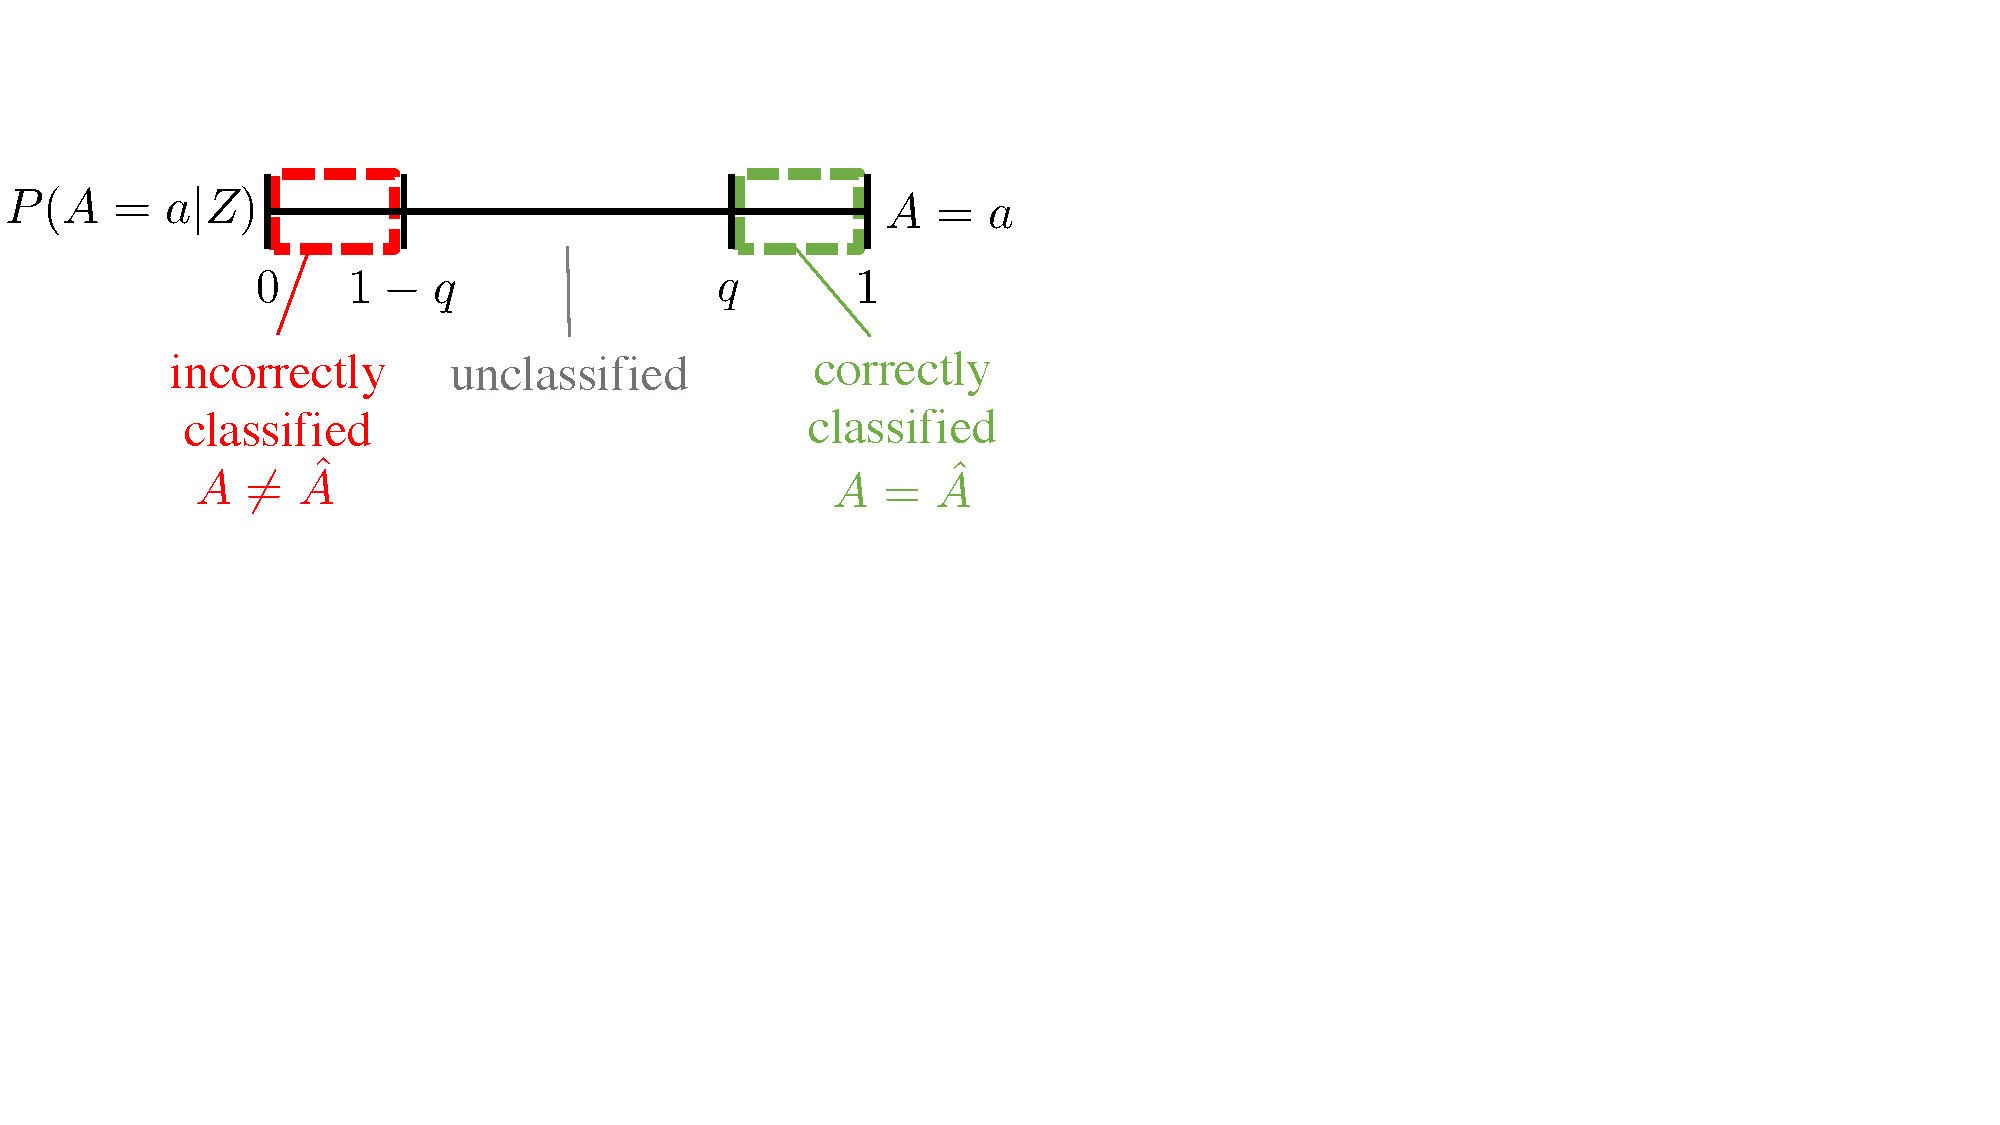
\includegraphics[width=0.6\linewidth]{threshold_rule.pdf}
\end{center}
%
where dashed boxes represent correct ($\hat{A}=A$, green) and incorrect classifications ($\hat{A}\ne A$, red), and the middle is unclassified.

We can use these predicted labels to estimate the mean group outcomes 
and demographic disparity by mimicking the simple estimator for 
group sample means difference, but imputing $\hat A$ for the
unknown $A$. This leads to the following estimator:

\begin{definition}
\label{def:thresholded_estimator}
Let $(Y_i, Z_i)_{i=1}^N$ be $N$ iid samples, $\{\hat{A}_i\}_{i=1}^N$ be the estimated labels according to the thresholding rule in Definition \ref{def:thresholding_rule}, and $\ind(S)$ be the indicator function for some set $S$. Then, the \textit{thresholded estimators} for mean group outcomes and demographic disparity are
%
\begin{align}
\hat{\mu}_{q}(u) & = \frac{\sum_{i = 1}^N \mathbb{I}(\hat{A}_i  = u)Y_i}{\sum_{i = 1}^N \mathbb{I}(\hat{A}_i  = u)}, u\in\{a,b\},  \nonumber \\
\hat{\delta}_{q} & = \hat{\mu}_{q}(a) - \hat{\mu}_{q}(b). \label{demo: est_race}
\end{align}
\end{definition}

% \begin{align}
% \hat{\delta}_{q} &= \hat{\mu}_{q}(a) - \hat{\mu}_{q}(b) \nonumber \\
% &= \frac{\sum_{i = 1}^N \mathbb{I}(\hat{A}_i  = a)Y_i}{\sum_{i = 1}^N \mathbb{I}(\hat{A}_i  = a)} -  \frac{\sum_{i = 1}^N \mathbb{I}(\hat{A}_i  = b) Y_i}{\sum_{i = 1}^N \mathbb{I}(\hat{A}_i  = b)} \label{demo: est_race}
% \\
% \hat{\delta}(x) = &\frac{\sum_{i = 1}^N \mathbb{I}(\hat{A}_i  = a)K_h(X - x)Y_i}{\sum_{i = 1}^N \mathbb{I}(\hat{A}_i  = a)K_h(X - x)} \nonumber\\
% &- \frac{\sum_{i = 1}^N \mathbb{I}(\hat{A}_i  = b)K_h(X - x) Y_i}{\sum_{i = 1}^N \mathbb{I}(\hat{A}_i  = b)K_h(X - x)} \label{cond_demo: est_race} \\
% \hat{\Delta} = &\sum_{j = 1}^{N'} \bigg\{\frac{\sum_{i = 1}^N \mathbb{I}(\hat{A}_i  = a)K_h(X_i - X^v_j)Y_i}{\sum_{i = 1}^N \mathbb{I}(\hat{A}_i  = a)K_h(X_i - X^v_j)} \nonumber\\ &- \frac{\sum_{i = 1}^N \mathbb{I}(\hat{A}_i  = b)K_h(X_i - X^v_j) Y_i}{\sum_{i = 1}^N \mathbb{I}(\hat{A}_i  = b)K_h(X_i - X^v_j)}\bigg\}  \label{adj_demo: est_race}
% \end{align}

% Here, we use kernel regression estimators to evaluate the conditional demographic disparity. But we may use many other supervised learning algorithms that can consistently estimate $\expect (Y \mid \hat{A} = w, X)$ and $\expect (Y \mid \hat{A} = b, X)$, e.g., the honest random forest (reference to Wager's paper).

% \subsubsection{Estimate protected attribute using weighted estimator}


\subsection{Weighted estimator}

The form of the thresholded estimators above shows clearly the use of a hard classification rule.
Under a probabilistic proxy model, this hard classification rule inevitably misclassifies some individuals,  given the intrinsic uncertainty in classifying the protected class.
Moreover, the threshold rule results in a group of unclassified individuals who are removed from the outcome disparity evaluation. 
To avoid these problems, we propose a new estimator that accounts for the soft classification generated by the proxy.

\begin{definition}
\label{def:weighted_estimator}
Let $(Y_i, Z_i)_{i=1}^N$ be defined as above.
Then, the \emph{weighted estimators} for mean group outcomes and demographic disparity are

\begin{align}
\hat{\mu}_W(u) & = \frac{\sum_{i = 1}^N \pr(A_i = a \mid Z_i)Y_i}{\sum_{i = 1}^N \pr(A_i = a \mid Z_i)}, u\in\{a,b\}  \nonumber \\
\hat{\delta}_W & = \hat{\mu}_W(a) - \hat{\mu}_W(b) \label{demo: weight}
\end{align}
\end{definition}

%\begin{align}
%\hat{\delta}_{W} = \hat{\mu}_{W}(a) - \hat{\mu}_{W}(b)
%=  -  \frac{\sum_{i = 1}^N P(A_i = b \mid Z_i)Y_i}{\sum_{i = 1}^N P(A_i = b \mid Z_i)}  \label{demo: weight}
% \\
% \hat{\delta}^{(a)}(x) = &\frac{\sum_{i = 1}^N P(A_i = a \mid Z_i)K_h(X_i - x)Y_i}{\sum_{i = 1}^N P(A_i = a \mid Z_i)K_h(X_i - x)} -  \nonumber\\
% &- \frac{\sum_{i = 1}^N P(A_i = b \mid Z_i)K_h(X_i - x)Y_i}{\sum_{i = 1}^N P(A_i = b \mid Z_i)K_h(X_i - x)} \label{cond_demo: weight} \\
% \hat{\Delta}^{(a)} = &\frac{1}{N}\sum_{j = 1}^N \bigg\{\frac{\sum_{i = 1}^N P(A_i = a \mid Z_i)K_h(X_i - X^v_j)Y_i}{\sum_{i = 1}^N P(A_i = a \mid Z_i)K_h(X_i - X^v_j)} \nonumber\\ &-  \frac{\sum_{i = 1}^N P(A_i = b \mid Z_i)K_h(X_i - X^v_j)Y_i}{\sum_{i = 1}^N P(A_i = b \mid Z_i)K_h(X_i - X^v_j)}\bigg \} \label{adj_demo: weight}
%end{align}

%Compared to the thresholded estimator, the weighted estimator acknowledges the uncertainty of the protected attribute given the predictors $Z$: the weighted estimator uses the proxy probabilities directly as the "soft" group membership as opposed to the hard group membership assigned by the thresholding rule. In the next section, we will show that this estimator has quite different theoretical property than the thresholded estimator.


\subsection{Toy examples}
\label{sec:toy_examples}

In this part, we use two hypothetical toy examples to demonstrate the intuition regarding when the thresholded estimator \eqref{demo: est_race} can overestimate the demographic disparity. In both examples, we consider evaluating the disparity of loan approval with respect to two races $A = a$ and $A = b$. However, the true race $A$ is unknown, so the geolocation $Z$ is used to estimate race. Suppose that there are only two neighborhoods where all people live in one neighborhood have high income and all people live in the other neighborhood have low income. We further assume that the high-income neighborhood is primarily occupied by the advantaged group $a$ and the low-income neighborhood is primarily occupied by the disadvantaged group $b$. Therefore, the thresholding rule with $q = 0.5$ classifies all people living in the high-income neighborhood as the advantaged group, i.e., $\hat{A} = a$,  and all people living in the low-income neighborhood as the disadvantaged group, i.e., $\hat{A} = b$.

\begin{table}
\centering
\caption{Lending policy of Example \ref{ex:income}, which always accepts high
income applicants and never low income applicants.
Each number in the table cells
represents the number of applicants who truly belong to race $a$ or $b$.
The percentages in parentheses represent the average loan approval
rate in that quadrant.} \label{table:toy1}
% \begin{threeparttable}
% \centering
\begin{tabular}{c c c}\toprule
& \multicolumn{2}{c}{True race} \\
Neighborhood & $a$ & $b$ \\
\midrule
 high income & 70 (100\%)          & 30 (100\%)\textsuperscript{i} \\
 low income  & 30 (0\%)\textsuperscript{ii} & 70 (0\%) \\
\bottomrule
\end{tabular}\\
% \begin{tablenotes}[flushleft]
% \item
\textsuperscript{i} Misclassified as race $a$ in high-income neighborhood.\\
% \item
\textsuperscript{ii} Misclassified as race $b$ in low-income neighborhood.
% \end{tablenotes}
% \end{threeparttable}
\end{table}

\begin{example}
\label{ex:income}
Consider an extreme lending policy: all people with high income get their loans approved, while all people with low income are rejected, no matter what their races are.
See Table \ref{table:toy1} for the illustration.
  Simple calculations show that the true demographic disparity $\delta = 40\%$ \footnote{$\delta = \frac{1}{100}(70\times 1 + 30\times 0) - \frac{1}{100}(30\times 1 + 70\times 0)  = 0.4$.} while the thresholded estimator $\hat{\delta}_{0.5} = 100\%$ \footnote{$\hat{\delta}_{0.5} = \frac{1}{100}(70\times 1 + 30\times 1) - \frac{1}{100}(30\times 0 + 70\times 0)  = 1$.}. Thus the thresholded estimator overestimates the demographic disparity. The reason for the overestimation is that the race proxy is correlated with the loan approval outcome because of the dependence between geolocation and socioeconomic status: people who live in the neighborhood primarily occupied by the advantaged group are also more likely to get loan approval because they have relatively high socioeconomic status, e.g.\ high income in this example. These people are classified as advantaged group because their neighborhoods are associated with high probability of belonging to the advantaged group. As a result, the thresholding rule misclassifies people who are from the disadvantaged group but get loan approval as the advantaged group. In this way, the thresholding rule leads to underestimates of the loan acceptance rate of the disadvantaged group. Analogously, the thresholding rule leads to overestimates of the loan acceptance rate of the advantaged group because it misclassifies people from the advantaged group but not likely to get loan approval as the disadvantaged group. Consequently, the misclassification of the protected attribute is dependent with the outcome, which ultimately leads to the overestimation of demographic disparity. The dependence between the misclassification and the outcome results from the \textit{inter-geolocation} outcome variation: the socioeconomic status, race proxy probabilities (i.e., race ratios), and loan acceptance rates vary across different neighborhoods such that the favorable outcome is positively correlated with the probability of belonging to the advantaged group.
\end{example}

\begin{table}
\centering
% \begin{threeparttable}
\caption{Lending policy of Example \ref{ex:affirmative_action}, with
affirmative action that favors the disadvantaged group over the advantaged
group at any given income level.\label{table:toy2}}
% \centering
\begin{tabular}{c c c}\toprule
& \multicolumn{2}{c}{True race} \\
Neighborhood & $a$ & $b$ \\
\midrule
high income & 70 (70\%) & 30 (80\%)\textsuperscript{i}\\ 
low income & 30 (20\%)\textsuperscript{ii} & 70 (30\%)\\ 
\bottomrule
\end{tabular}\\
% \begin{tablenotes}[flushleft]
% \item
\textsuperscript{i} Misclassified as race $a$ in high-income neighborhood.\\
% \item
\textsuperscript{ii} Misclassified as race $b$ in low-income neighborhood.
% \end{tablenotes}
% \end{threeparttable}
\end{table}


\begin{example}
\label{ex:affirmative_action}
  Now consider a hypothetical lending policy with affirmative action that approves the disadvantaged group with higher rate than the advantaged group with the same income level. But overall people with high income are still more likely to be accepted. See Table \ref{table:toy2} for a concrete example. Simple calculations show that the true demographic disparity $\delta = 10\%$ \footnote{$\delta = \frac{1}{100}(70\times 0.7 + 30 \times 0.2) - \frac{1}{100}(30\times 0.8 + 70 \times 0.3) = 0.1$.}, which means that the disadvantaged group overall has lower chance to get loan approval due to their population concentration in the low-income neighborhood. However, the thresholded estimator gives  $\hat{\delta}_{0.5} = 46\%$ \footnote{$\hat{\delta}_{0.5} = \frac{1}{100}(70\times 0.7 + 30 \times 0.8) - \frac{1}{100}(30\times 0.2 + 70 \times 0.3) = 0.46$.} that overestimates the demographic disparity. The reason for the overestimation is that the the disadvantaged group have higher approval rate than their neighbors from the advantaged group. As a result, misclassifying part of the disadvantaged group as the advantaged group raises the average approval rate for the advantaged group. Similarly, misclassifying part of the advantaged group as the disadvantaged group lowers down the average approval rate for the disadvantaged group. Consequently, the misclassification of the protected attribute is also dependent with the outcome and ultimately leads to overestimation of demographic disparity. In contrast to Example \ref{ex:income}, the dependence between the misclassification and the outcome results from the intra-geolocation outcome variation: people from different protected groups living in the same locations have different chance of getting the favorable outcome.
\end{example}

In both examples, the protected attribute misclassification made by the thresholding rule is not uniformly at random. Instead, the misclassification shows systematic pattern with respect to the outcome either due to the inter-geolocation outcome variation (Example \ref{ex:income}) or intra-geolocation outcome variation (Example \ref{ex:affirmative_action}). In Section \ref{sec:theorems}, we will formalize the main intuition in these two examples and show that the interplay of the two bias sources captured by these two examples determines the overestimation or underestimation of the thresholded estimator. In Section \ref{sec:numerics}, we will further identify the specific bias source that accounts for the estimation bias of the thresholded estimator in a mortgage data set.
